\documentclass[english]{siamltex}
\usepackage{graphicx}
\usepackage{amsmath}
\usepackage{amssymb}
\usepackage{amsfonts}
\usepackage{latexsym}
\usepackage{pstricks}\usepackage{tikz,pgflibraryplotmarks}

\newcommand {\R}    {{\rm I\!R}}
\newcommand {\bu}   { {\bf u} }          			% discrete flow field
\newcommand {\buref}   { {\bf u}_{\text{ref}} } 	% discrete reference flow field
\newcommand {\bugt}   { {\bf u}_{\text{gt}} } 	% discrete ground truth flow field
\newcommand {\bfx}  { {\bf x} }
\newcommand {\bfd}   { {\bf d} }
\newcommand {\bfe}   { {\bf e} }

\newcommand {\bfs}   { {\bf s} }
\newcommand {\bsgt}   { {\bf s_\text{gt}} }
\newcommand {\bfu}   { {\bf u} }
\newcommand {\bfq}   { {\bf q} }
\newcommand {\bfp}   { {\bf p} }
\newcommand {\bfz}   { {\bf z} }
\newcommand {\bfy}   { {\bf y} }
\newcommand {\bfk}   { {\bf k} }


\newcommand {\bfK}  { {\bf K} }
\newcommand {\bfP}  { {\bf P} }
\newcommand {\bfA}  { {\bf A} }
\newcommand {\bfB}  { {\bf B} }

\newcommand {\bfG}  { {\bf G} }
\newcommand {\bfF}  { {\bf F} }
\newcommand {\bfI}  { {\bf I} }


\newcommand {\vu}  { {\vec {\bf  u}} }   % continuous flow field
\newcommand {\vuref} {\vu_{\text{ref}}}  % continuous reference flow field
\newcommand {\vq}  { {\vec {\bf  q}} }
\newcommand {\ve}  { {\vec {\bf  e}} }
\newcommand {\vh}  { {\vec {\bf  h}} }
\newcommand {\vx}    {\vec {\bf x}}     
\newcommand {\bx}    {{\bf{x}}}     
\newcommand {\bfr}    {{\bf{r}}}     

\newcommand {\bflambda}    {{\boldsymbol{\lambda}}}     



\renewcommand {\diag}	 { \mathrm{diag} }
\newcommand {\blambda}	 { {\boldsymbol \lambda} }
\newcommand {\bmu}    	 { {\boldsymbol \mu} }
\newcommand {\zero}   	 { {\bf 0} }
\newcommand {\gb}      	 { {\bf g} }
\newcommand {\bnabla}	 { { \boldsymbol \nabla} }
\newcommand {\btheta}	 { { \boldsymbol \theta} }
\newcommand {\balpha}	 { { \boldsymbol \alpha} }
\newcommand {\bfxi}		 { { \boldsymbol \xi} }
\newcommand{\hf}		 {\frac12}
\newcommand{\hx}[1]		{{\ensuremath{h^x_{\scriptscriptstyle #1}}}}
\newcommand{\hy}[1]		{{\ensuremath{h^y_{\scriptscriptstyle #1}}}}
\newcommand{\hz}[1]		{{\ensuremath{h^z_{\scriptscriptstyle #1}}}}
\newcommand{\E}			{\vec{E}}
\newcommand{\A}			{\vec{A}}
\renewcommand{\H}		{\vec{H}}
\newcommand{\J}			{\vec{J}}
\newcommand{\F}			{\vec{F}}
\newcommand{\M}			{\vec{M}}

\newcommand{\s}{\vec{s}}
\newcommand{\h}{\vec{h}}

\newcommand{\sig}{\sigma}
\newcommand{\nn}{\vec{n}}
\renewcommand{\div}{\nabla\cdot\,}
\renewcommand{\grad}{\ensuremath {{\bf{ \nabla}}}}
\newcommand{\curl}{\ensuremath{{\nabla}\times\,}}

\newcommand{\alert}[1] {\textcolor{red}{#1}}
\newcommand{\jen}[1] {\textcolor{blue}{#1}}
\newdimen\iwidth\iwidth=30mm
	\newcommand{\rottext}[1]{\rotatebox{90}{\hbox to 30mm{\hss #1\hss}}}


\newcommand{\rme}{\rm{e}}


% JENNS NewCommands
\newcommand{\bA}  { {\bf A} }      % transport matrix
\newcommand{\bB}  { {\bf B} }      % matrix for initial condition of hyperbolic problem, B=[T;0;...;0]
\newcommand{\bc}  { {\bf c} }      % time series of concentration, c = [c1,...,cN]
\newcommand{\bI}  { {\bf I} }      % identity matrix
\newcommand{\bF}  { {\bf F} }      % tomography matrix
\newcommand{\bG}  { {\bf G} }      % image gradient, G = dT = GRAD( T * s)
\newcommand{\bT}  {\text{{\bf T}}} % push forward matrix
\newcommand{\bM}  {\text{{\bf M}}} % interpolation matrix
\newcommand{\bfJ}  {\text{{\bf J}}} % interpolation matrix

\newcommand{\JJ}  {\mathcal{J}}    % objective functional
\newcommand{\cD}  {\mathcal{D}}    % data misfit
\newcommand{\CR}  {\mathcal{R}}    % regularization functional
\newcommand{\CRflow}  {\mathcal{R}^{\text{flow}}}    %  flow regularization functional
\newcommand{\CRsat}   {\mathcal{R}^{\text{s}}}     %  saturation regularization functional
\newcommand{\CF}  {\mathcal{F}}    % continuous tomography operator
\newcommand{\sh}  {\texttt{s}}     % discretized initial slowness
 \newcommand{\DIVh}   {{\textsf{DIV}}}  % discretized divergence operator
%\newcommand{\DIVh}   {(\nabla \cdot)_h}  % discretized divergence operator
\newcommand{\CURLh}  {{\textsf{CURL}}} % discrete curl operator
%\newcommand{\CURLh}  {(\nabla \times)_h} % discrete curl operator
\newcommand{\GRADh}  {{\textsf{GRAD}}} % discrete gradient operator
% \newcommand{\philone}  {\phi_{\ell_1}} % l1 curl regularizer
% \newcommand{\philtwo}  {\phi_{\ell_2}} % l2 curl regularizer
\newcommand{\W}{\text{\bf W}}


\def\kronecker{\raisebox{1pt}{\ensuremath{\:\otimes\:}}} 
\sloppy


\begin{document}

\title{Geophysical imaging of fluid flow in porous media}
\author{J. Fohring, E. Haber and L. Ruthotto}


\maketitle
\begin{abstract}
	Imaging and prediction of fluid flow in the subsurface provides information that is crucial for decision making processes in fields such as groundwater management and enhanced oil recovery. The flow of an injected fluid through a reservoir depends primarily on the hydraulic conductivity, which is in general unknown or only known with low accuracy. A common way of imaging the flow is thus to intelligently modify the hydraulic conductivity model, simulate the fluid flow and geophysical imaging data that approximately match the observations over time. This process is also known as history matching. As the imaging process is a highly underdetermined inverse problem, we propose a new technique that avoids estimation of hydraulic conductivities. Instead, our approach directly estimates the flow field and initial distribution of the fluid from a time series of geophysical imaging data.
	
	Our method combines the flow equations with geophysical imaging  to form a single inverse problem,  where the unknowns are the initial state of the reservoir and the flow field. We discuss consistent discretization techniques, tailor specific regularizations, and use a modification of the variable projection method to solve the discrete optimization problem. We demonstrate the potential of our method on a model problem and show that our approach yields an improved flow estimate as well as an improved image quality. Finally, we show that the estimated flow field allows for the reconstruction of  the subsurface structure.

\end{abstract}
\section{Introduction} % (fold)
\label{sec:introduction}


Managing fluids in porous media is an important field
of reservoir and civil engineering~\cite{GerritsenDurlofsky2005} as it aids in 
more efficient recovery of water, oil, and gas.
In principle, the dynamics of the reservoir are governed
by the flow in porous media equations~\cite{ChenHuanMaBook}.
Given reservoir parameters and initial conditions,
these equations can predict the time evolution of flow within the
reservoir and therefore aid in its management.
 
One major challenge of fluid management stems from the large number
of unknown parameter functions in the flow equations.
Quantities such as porosity, hydraulic conductivity,
mobility functions, and capillary pressure functions
are in many cases spatially dependent and  unknown.
These parameter functions are typically sparsely sampled 
 in space and have a  multi-scale 
structure~\cite{WangTartakovsky13}. To alleviate this problem, historic
flow data can be used to estimate the unknown
parameters. Such a process is often referred to as history
matching~\cite{DeanChen2011,OliverBook2008}.

The basic idea of history matching is to intelligently 
modify the physical properties of the reservoir such 
that simulated flow data fits measured data. Technically,
this process is rather challenging as it involves 
the solution of the forward problem (reservoir simulation),
the computation of the gradients of the simulator with
respect to the parameters, and the solution of a regularized
optimization problem for the coefficients. An excellent
review of the process can be found in~\cite{DeanChen2011}.

Even though it is possible to estimate
some physical properties that fit the flow data,
these physical properties can be a highly inaccurate
representation of the reservoir.
The reason being that there is a large null space of
 the inverse problem associated
with a highly sparse sampling of the reservoir in space.
To overcome this, subspace techniques have been
used~\cite{DeanChen2011,GerritsenDurlofsky2005,SarmaDurlofskyAziz2007,Oliver01}.
In these techniques one restricts
the physical properties to ``live'' in a small subspace
spanned by a (relatively) small number of vectors.
This approach decreases the variance in the recovery
by increasing the bias of the estimated physical 
properties~\cite{tensiam}.

A different approach to reduce the variance of the
recovered earth models is to simply add data and further
sample the reservoir. While this
is clearly one of the better ways to reduce the uncertainty
in the recovery, it is not practical as it is
unlikely that many more wells are drilled just to improve
the simulation capability.
However, while direct measurements are difficult
and expensive to obtain, indirect measurements
of reservoir properties are cheap and relatively
easy to get. Such measurements include time lapse
seismic and electromagnetic imaging data 
\cite{Lumley2001,VascoEtAl2004}. 
Our interest in this paper is given to first arrival
seismic tomography data commonly used in reservoir management.

In the field of reservoir monitoring using geophysical
methods is rather new~\cite{FahimuddinPhd,GosselinEtAl,NennaEtAl2011,MezghaniEtAl,EmerickReynolds12,TraniPhd}. 
All work known to us decouples the imaging and the flow, recovering the images without considering
the flow equations.
This process has a
major shortcoming. Since geophysical imaging is almost always
ill-posed, the accuracy of the imaging is typically low. Estimating the
flow from the images can therefore yield inaccurate 
and biased estimates.

In this paper we suggest a new methodology to combine the geophysical imaging
with flow. We  show how to improve the imaging using the flow and at the
same time improve the recovery of the flow, resulting in the  ability to better forecast
the fluid motion in the ground.
We choose  tracer advection as our model flow problem. 
While this is simpler than more realistic two or three phase flow models, it has many similar properties
that serve us well as a model problem.


 
While our approach is new, it has many similarities to the
approach taken to solve the problem of super-resolution~\cite{CHN06} and imaging with optical flow~\cite{BruneMaurerWagner2009}, a common problem in computer graphics. Super-resolution uses
a number of blurred images  shifted in space 
in order to recover a single high resolution image. 
Similar to super-resolution both the displacement (motion) and
the initial conditions are in general unknown. The main differences
between super-resolution and the problem at hand are that
our flow model is substantially more complex and the imaging
technique is more difficult as compared with simple image deblurring.
As a result, we develop a  new regularization strategy to be used for
the flow estimation.


\medskip

The paper outlines as follows. In Sec.~\ref{sec:mathematical_formulation}, we  briefly introduce our notation, the mathematical formulation of reservoir simulation, the borehole seismic tomography survey, and define our approach to estimating the subsurface flow and initial state of the reservoir from tomography data.
We define a new objective functional to be minimized with respect to both the flow velocity field and the initial change in seismic slowness.
In Sec.~\ref{sec:numerical_methods_for_the_forward_problem}, we describe the discretization of the
forward probleand the inverse problems, keeping in mind stability and differentiability that are needed for the optimization.
In Sec.~\ref{sec:numerical_optimization} we discuss a numerical optimization method for solving the discrete inverse problem. 
Finally, we present numerical examples in Sec.~\ref{sec:numerical_examples}.

\bigskip

% section introduction (end)

\section{Mathematical formulation} % (fold)
\label{sec:mathematical_formulation}

In this section we introduce our notation for the governing equations 
of  flow simulation and borehole seismic tomography, concentrating on the problem of tracer flow~\cite{ChenHuanMaBook}. 
A similar approach can be used for more complex flow (i.e. multiphase flow) where the
elliptic and hyperbolic problems are non-linear. However, 
in this paper we concentrate on a simple problem allowing us to
demonstrate the techniques at hand.

We then discuss our approach for the solution of the inverse problem which combines the tracer flow equations and tomographic imaging, and discuss our choice of an appropriate
regularization strategy for the solution of the problem.



\subsection{Tracer Dynamics} % (fold)
\label{sub:reservoir_simulation}

We start by considering the tracer flow equations outlined in~\cite{ChenHuanMaBook}. These equations describe the transport of a solute in a fully saturated fluid phase with the assumption that fluxes due to dispersion and diffusion are small relative to the advective transport of the solute.
We consider the flow of a tracer with concentration $c$ (volumetric fraction in the fluid phase), in a fluid of density $\rho$ 
%where $\phi$ is the porosity of the porous medium,
\begin{subequations}
\label{floweq}
\begin{eqnarray}
 \label{eq:flow}
&&\frac{\partial( c \rho)}{\partial t} + \div c \rho \vu  = 0,\\
\nonumber
 &&\text{ subject to } c\rho(0,\vx) = c_0\rho(\vx),
\end{eqnarray}
where the flow field $\vu$ satisfies 
\begin{eqnarray}
\label{eq:flowp}
&&  \div  \vu =   q \\ % \mu^{-1}\bfK(\bfx) \grad p
\label{eq:flowu}
&& \vu =  \bfK(\vx)  \grad p \\
\label{eq:incond}
&&  p(0,\vx) = p_0(\vx).
\end{eqnarray}
\end{subequations}
accompanied with either Dirichlet or Neumann boundary conditions for the pressure, $p$.

% EH-note
% In most books they write the problem as
% $$ \phi \rho_{t} + \div \vu \rho = 0 $$
% where $\phi$ is the porosity and $\vu = -K \grad p$
% Now since \phi does not change in time we can re-define a new variable $\hat \rho = \phi \rho$
% and write
% $\hat \rho_{t} + \div \hat \vu \hat \rho = 0$
% where $\hat \vu = -\phi^{-1} K \grad p$.

Note that in this formulation the unknowns are the  pressure $p$ and the tracer concentration $c$.
% and that there is no tracer injected. 
The source term $q$ is given, and the conductivity parameter function  $\bfK(\vx)$ is assumed to be known 
for the simulation to be carried out. 
However, in practice,  $\bfK(\vx)$ is unknown, or known only to very low accuracy. Therefore, solving the forward problem gives only qualitative information about the flow and in particular impedes accurate predictions.
  Therefore, in the remainder of the paper, we focus on estimating 
  the flow field $\vu$ and the initial tracer concentration $c$ from tomography by data taking the flow equations,~\eqref{floweq}, into consideration.
  We later show that given $\vu$ we can also estimate the hydraulic conductivity. However, the velocity is directly related to the fluid flow and therefore we prefer to estimate it instead.

 
\subsection{Borehole seismic tomography} % (fold)
\label{sub:geophysical_imaging}
Boreholes seismic surveys can be conducted in order to monitor the progression of the tracer as it flows within a porous media. 
The seismic tomography survey generates 
data that can be inverted to provide an image of flow within the subsurface. 
We therefore outline the experimental set-up and introduce a mathematical 
formulation of first arrival seismic travel times.   



A typical tomography experiment places $n_s$ sources on one side of the region to be imaged 
 and $n_r$ receivers on the other. Travel times from source to receiver constitute the 
measured data, and the ultimate goal is to recover the changes to the distribution of physical properties 
generating changes in these data. A schematic of the  seismic experiment is illustrated in Fig.~\ref{figTomo}. 
\begin{figure}[t]
\begin{center}
	\input{fig1/boreholeTomography.tex}
\caption{Tomography setting: Sources and receivers are placed in two boreholes and the travel times of an acoustic wave traveling along adjoining ray paths are measured.
\label{figTomo} }
\end{center}
\end{figure}

Mathematically, the travel time data are given by integrating the inverse of the acoustic velocity, also know as the slowness, $s(t,\vx)$, over a ray path.
The travel time along the ray path $\Gamma_{j,k}$ from the $j$th source to the $k$th receiver is  given by 
\begin{equation}\label{eq:tomo}
\bfd_{j,k}(t) =  \int\limits_{\Gamma_{j,k}} s(t,\vx)\, d\ell.
\end{equation}
where $s \in {\cal S}$ is the slowness model that belongs to some subspace, ${\cal S}$, that is characterized later.
Assuming that the ray path is independent of the slowness (this is true for small perturbations
in the slowness field), the problem can be cast as a linear inverse problem for $s(t,\vx)$ given $\bfd(t)$.
Given noisy data measured at times $(t_{0},\ldots,t_{n})$  we
can write 
\begin{eqnarray}
\label{eq:forim}
\CF s(t_{j},\vx) + \epsilon_{j}  = \bfd(t_{j})
\end{eqnarray}
where $\bfd$ is a  ${n_s \times n_r}$ vector of real numbers,  $\CF:{\cal S} \rightarrow \R^{n_s \times n_r}$ is the forward mapping,  and $\epsilon$ is
a random vector assumed to be identically independently distributed. 

\subsection{Variational imaging of fluid flow problems} 
\label{sub:derivingTheObjectiveFunctional}

In order to generate a  forecast of the tracer flow within a reservoir the initial tracer distribution and fluid velocity field 
will be estimated given seismic tomography data and the flow equations~\eqref{eq:flow}.


Before discussing the use of imaging for flow estimation, we need to discuss the
connection between the tracer $\hat c = c \rho$ and the seismic slowness $s$.
Clearly, the two are different physical properties and have different units, however,
we assume that the connection $s(\hat c)$ exists.

In some cases, the relationship between $s$ and $\hat c$ can be determined empirically~\cite{GosselinEtAl},
though this requires  elaborate laboratory work and cannot be generated for the general case.

It is interesting to note that in the case that the flow is divergence free,
one does not need to know this relation explicitly. Note that if $\div \vu = 0$ then
$$\hat c_{t} + \div (\hat c \vu)  = \hat c _{t} + \vu^{\top} \grad \hat c = 0 $$ 
and therefore
$$ \frac{\partial}{\partial t}s(\hat c ) + \div (s(\hat c) \vu) 
= s_{ \hat c} \hat c _{t} +  \vu^{\top} s_{ \hat c} \grad \hat c
= s_{ \hat c} \left(\hat c _{t} + \vu^{\top} \grad \hat c \right) = 0. $$
For the problem at hand~\eqref{eq:flowp} typically has a very sparse right hand side with delta functions for injection and extraction points. Therefore, the flow field is divergence
free almost everywhere.
Thus, we can assume that the transport equation describing the flow of the tracer can also be used for the ``transport'' of the slowness.

\bigskip

The problem  of estimating the flow from seismic data is 
commonly referred to as \emph{seismic  history matching} (see
\cite{Lumley2001,GosselinEtAl,FahimuddinPhd} and references within). 
All algorithms known to us attempt to recover the conductivity and other reservoir parameters
in order to use them for flow simulation. These approaches require knowing the connection between
$\hat c$ and $s$ and do not incorporate the fluid model into the seismic reconstructions in order to improve the images.
Our approach is different; rather than recovering reservoir parameters we aim to
recover the velocity field directly. By doing so we are then able to march the initial tracer along in time 
and forecast the tracer's dynamics. 

\bigskip

Given the flow equations, the seismic data, and the connection between them, we propose 
to solve the following variational problem to jointly estimate the flow field and initial slowness
\begin{subequations}
\begin{eqnarray} 
\label{eq:J}
\min_{s_{0},\vu} && \JJ(\vu,s_0) = \hf  \sum_{i=1}^n \left\|  \CF  s(\vx,t_i) - {\bf d_i}  \right\|^2 + \CRflow(\vu) +  \CRsat(s_0)  \\
\label{eq:c}
\text{subject to } &&  s_t + \div (s \vu ) = 0, \quad s(0,\vx) = s_0,\quad \div \vu = q.
 \end{eqnarray}
 \end{subequations}
The first term measures the misfit in~\eqref{eq:forim} in a least-square sense. Minimizing $\JJ$ under the flow constraints
yields a velocity field and slowness distribution which fits the tomography data. However, since both the tomography
 and flow estimation problems are ill-posed, regularization is needed. 
We define $\CRflow(\vu)$ as a regularization 
functional on the velocity field, and $\CRsat(s_{0})$ as a regularization functional for the initial slowness.

While our approach for the recovery is a frequentist one it can be interpreted as a Maximum A-Posteriori (MAP) Bayesian
estimate, where the first term, the misfit, is the negative log-likelihood and the second and third terms
are the negative logs of the priors for the flow and initial slowness. 

The question is, what regularization should be used for the velocity and slowness?
 We propose the following regularization for $\vu$:
 	\begin{equation} \label{eq:regularizer}
	 \CRflow(\vu ) = \int   \alpha_1 \  \phi(\curl \vu)\  +  \frac{\alpha_2}{2}\ w(\vx)\ |\vu - \vuref|^2 d\vx,
	\end{equation}
	where the first term  penalizes the {\bf curl} of the flow field and  the second term seeks to minimize the difference between the recovered velocity, $\vu$, and a reference velocity, $\vuref$.
The parameters $\alpha_1,\alpha_2>0$ balance the contribution of both terms.

We choose to regularize the {\bf curl} of the flow, since the divergence and the {\bf curl} complement
each other. Given that the {\bf div} of the flow field is set by the constraint~\eqref{eq:c}
we choose to regularize only over its  orthogonal complement.
To choose the penalty function $\phi$, we note that
sharp contrasts in hydraulic properties of different rock units are common; for example see visualization of the $\curl \vu$ in left column in Fig.~\ref{fig:reconResults}.  The velocity field
is $\vu = \bfK \grad p $ with $\div \vu = q$ and since
$$ \curl \vu = \curl (\bfK \grad p) = \grad p \times \grad \bfK $$
  the {\bf curl} of the flow field 
has tangential discontinuities where $\bfK$ has jumps.
Thus, assuming that $\bfK$ is piecewise constant, the curl of the velocity 
is expected to be sparse. 
We therefore employ the convex function 
$$\phi (c)=  \sqrt{c^2 + \epsilon}, $$ 
which is an approximation to the $\ell_1$-norm on the {\bf curl}. 
 % By appropriate choices of  $\alpha_i\geq 0$ the functional 
% $\CRflow$ allows individual regularization of the {\bf curl} and the deviation of the velocity field from the reference field. 

The reference model, $\vuref$, is included in order to incorporate prior information about the subsurface. The weighting function $w(\vx)$ quantifies the confidence in $\vuref$; see~\cite{OldenburgPratt2007}. One option to compute $\vuref$ is by solving~\eqref{eq:flowp} and~\eqref{eq:flowu} using a reference 
conductivity model $\bfK_{0}$  constructed from a priori borehole data as described in Sec.~\ref{sec:numerical_examples}.  In this case, $w(\vx)$ is large close to the boreholes and smaller as the distance from the known drill site grows.


\bigskip

The initial slowness can also be discontinuous and therefore we use smoothed
Total Variation~\cite{ahh} as a regularization term, given by	
\begin{equation}
		\CRsat(s_0) = \beta \int  \phi(|\grad s_0|) \ d\vx.
\end{equation} 
		
Finally, the regularization parameters $\alpha_{1}$, $\alpha_{2}$ and $\beta$ are chosen such that the data misfit is approximately equal to the norm of the noise, which is in general unknown,\cite{parker}. Therefore, a cooling strategy that starts with large regularization parameters which are decreased incrementally until a reasonably small data misfit is achieved is used to calibrate the model in our numerical experiments; see Sec.~\ref{sub:sequential_reconstruction}.

Given the data misfit and regularization operators we now discuss the discretization and the
numerical solution of the problem.

\section{Discretization} % (fold)
\label{sec:numerical_methods_for_the_forward_problem}

In this section we derive a numerical discretization of the forward simulation of travel time data, the inverse estimate of the subsurface flow field, 
and the regularization operators.   
This section is divided into 
three parts;  the discretization of the flux mass-balance, conservation law~\eqref{eq:flow}, and the tomography experiment. 

For simplicity, we restrict the presentation to the two-dimensional setting, assume that the computational domain is rectangular $\Omega = [0,L_{1}]\times [0,L_{2}]$, and is divided into $m_{1}$ by $m_{2}$ rectangular
cells of edge length $h_{1}=L_{1}/m_{1}$ and $h_{2} = L_{2}/m_{2}$. 

Next, the vector field $\vu$ and the initial slowness $s_{0}$ are discretized. Since 
vector operators such as the {\bf curl} and divergence are used, a Marker and Cell (MAC) grid is chosen~\cite{fletcher} 
(see Fig.~\ref{fig:stag})
where $\vu = [\vu_{1},\vu_{2}]$ is discretized by the staggered grid functions $\bfu = [\bfu_{1}^{\top}, \bfu_{2}^{\top}]^{\top}$
on cell faces. This yields an approximation of the divergence in the cell-centres using short differences, which are sensitive to highly oscillatory functions. Therefore the discretization of the divergence does not introduce an additional nullspace which might lead to instabilities of the discrete saddle point problems arising in the numerical optimization scheme introduced below in Sec.~\ref{sec:numerical_optimization}; see also~\cite{fletcher,sekw}.

The initial slowness $s_{0}$ is discretized using a cell-centred grid function $\bfs_{0}$.
Given the discretization of the slowness and the velocity we now discuss the discretization of
the different components of the objective functional~\eqref{eq:J} and the constraints~\eqref{eq:c}.
\begin{figure}[t]
\begin{center}
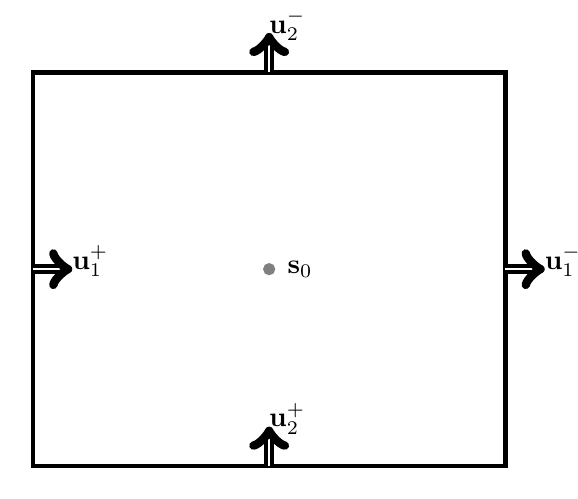
\begin{tikzpicture}[scale=1]
 	\draw[ultra thick]  (0,0) -- (6,0) -- (6,5) -- (0,5) -- cycle;
	\draw[black,ultra thick,double,->] (0,2.5) -- (0.5,2.5);
	\draw[black,ultra thick,double,->] (6,2.5) -- (6.5,2.5);
       \draw[black,ultra thick,double,->] (3,0) -- (3,0.5);
       \draw[black,ultra thick,double,->] (3,5) -- (3,5.5);
       
       %\draw[blue,ultra thick,double,->] (2,-2.5) -- (1,-2.7);
       %\draw[blue,ultra thick,double,->] (3.5,0) -- (3.5,1);
       %\draw[blue,ultra thick,double,->] (6,-2) -- (7,-2);
      \draw [gray,fill] (3,2.5) circle (2pt);
       \pgfputat{\pgfxy(3,2.5)}{\pgfbox[left,center]{\ \ $\bfs_{0}$}};
      \pgfputat{\pgfxy(0.5,2.6)}{\pgfbox[left,center]{$\bfu_{1}^{+}$}};
      \pgfputat{\pgfxy(6.5,2.6)}{\pgfbox[left,center]{$\bfu_{1}^{-}$}};
      
      \pgfputat{\pgfxy(3.0,0.6)}{\pgfbox[left,center]{$\bfu_{2}^{+}$}};
      \pgfputat{\pgfxy(3.0,5.6)}{\pgfbox[left,center]{$\bfu_{2}^{-}$}};
      

       \end{tikzpicture}
\caption{A control volume. \label{fig:stag}}
\end{center}
\end{figure}

\subsection{Discretization of the flux-balance conservation} % (fold)
\label{sub:mass-balance}

A finite volume discretization of the flux-balance equation $\div \vu = q$ on a staggered grid
is obtained by using the divergence theorem; see~\cite{ha} for details. 
Referring to Fig.~\ref{fig:stag}, the divergence over a cell with dimensions
of $h_{1} \times h_{2}$ in our mesh can be expressed as
$$ (\div \vu)_{\rm cell} \approx {\frac { h_{2}(\bfu_{1}^{+} - \bfu_{1}^{-}) +  h_{1}(\bfu_{2}^{+} - \bfu_{2}^{-})}{h_{1}h_{2}}} $$
where the $\bfu_{i}^{+}$ is flux into the cell and $\bfu_{i}^{-}$ is the flux out of the cell in $i$th coordinate direction.
This discretization leads to the following standard discretization of the divergence
\begin{equation}
\label{diveq}
 \DIVh\ \bfu = \bfq \text{, where }
	\DIVh = \begin{pmatrix}
					{\bf I}_{m_{2}} \kronecker {\bf d}_{m_{1}+1}^{m_{1}} &   {\bf d}_{m_{2}+1}^{m_{2}} \kronecker
					 {\bf I}_{m_{1}}
				\end{pmatrix}
\end{equation} 
with ${\bf I}_m \in \R^{m \times m}$ denoting the identity 
matrix and where ${\bf d}_{m+1}^m \in \R^{m \times m+1}$ is a short finite difference matrix; see~\cite{ModSiamBook} for more details about the implementation.
The discrete divergence operator maps from faces of the mesh to cell-centers.


\subsection{A Particle-In-Cell method for flow simulation} % (fold)
\label{sub:particle-in-cell}
The  hyperbolic conservation law~\eqref{eq:flow} can be discretized in a number of ways. One option is to use explicit Eulerian techniques such as upwinding, Lax-Wendroff or Lax-Friedrichs~\cite{ascher}.
However, explicit techniques  suffer from one main shortcoming: since the velocity of the equation is
unknown, one has to monitor the time step making sure stability is maintained.
Monitoring and adjusting the time step can add enormous complexity to the optimization technique used to recover the velocity.
Methods such as upwinding and other flux limiters have another shortcoming: they are not differentiable
with respect to the velocity and therefore simple optimization techniques can run into difficulties if care
is not taken. One has the option of using implicit methods which require the solution of linear systems at
every time step, or using semi-Lagrangian techniques. Semi-Lagrangian techniques are particularly attractive
for this application as they are explicit, unconditionally stable and can be easily made differentiable.
Semi-Lagrangian methods can suffer from low accuracy, however for our application where the
velocity field is inaccurate, working with highly accurate discretizations is usually computationally 
wasteful. 
We therefore discuss a Particle-In-Cell (PIC) method  that can also be interpreted as a semi-Lagrangian technique, for the solution of the problem.
We first describe a PIC method for computing the evolution of the slowness $s$  given a flow field $\vu$ and initial slowness $s_0$ using the hyperbolic equation~\eqref{eq:flow}. As discussed, PIC methods are mass-conserving,
 unconditionally stable, and can be made continuously differentiable with respect to both $\vu$ and $s_0$. 
The idea of using PIC methods for the solution of conservation laws is not new and was proposed in~\cite{PIC55}. 
Recently, PIC methods have emerged in computer graphics 
\cite{BridsonPIC} and in flow in porous media~\cite{RoubinetDreuzyTartakovsky13}
and have been designed to deal with higher order integration methods in space-time as well as 
other geometrical constraints.

To use PIC methods, a particle $\bfx_j$ is associated with the midpoint of the $j$th grid cell. 
The particle is assigned a value $\bfs_{j} = s_0(\vx_j)$, and the advection of 
the particle $\bfx_j$ is described by the following ODE
\begin{equation}\label{eq:characteristics}
	\frac{\partial\bx_j(t)}{\partial t} = \vu(x).
\end{equation}
Using a midpoint quadrature rule, the particle's position after the first time step approximately 
\begin{equation}
	\bx_j(t_{1}) = \bx_j(0) +  \Delta t (\bfA_{f}^{c} \bu)_j + {\cal O}({\Delta t}^2),
\end{equation}
where $\bfA_{f}^{c}$ denotes an averaging operator from faces (where the velocity resides)
to cell centers.
Thus, the position of the particle at a later time is easily computed given a time step and velocity field. 

Since the new position will in general not be the mid-point of a cell, the value $\bfs_{j}$ is 
distributed to the closest surrounding points  as illustrated in Fig.~\ref{figSL}. 
To compute the distribution weights we use bilinear basis functions, although higher order interpolation techniques can and have been applied~\cite{BridsonPIC}.
Thus, the slowness field $\bfs_{i+1}$ at time $t_{i+1} = t_{i} +\Delta t$ is given by
\begin{equation}
	\bfs_{i+1} = \bT(\Delta t\bu) \bfs_{i},
\end{equation}
where $\bT(\Delta t\bu)$ denotes the push-forward matrix containing the values of the bilinear hat functions 
 associated with the particles at the grid points. Since the value of each particle is spread 
 between neighboring cell-centers, this construction guarantees exact mass preservation as long as no flux exits at the boundaries of the computational domain.  Using the  push forward matrix, the time-stepping process is then
 \begin{eqnarray}
 \label{eq:dhcl}
 \bfs_{i+1} = \bT(\Delta t\bu) \bfs_{i} = \bT(\Delta t\bu)^{i+1} \bfs_{0}.
 \end{eqnarray}
The slowness at the $(i+1)$th time step is therefore a pushed-forward version of $\bfs_0$, where the path the particle takes is piecewise linear.
Although it is possible to obtain 
curved paths, this adds complexity to the method and makes the method more difficult to work with. This difficulty arises in the inverse problem because derivatives of  the objective function and the constraints are required.  


Assuming the velocity field is constant in time, the evolution of the slowness is computed by repeating~\eqref{eq:dhcl} for all time steps
\begin{eqnarray*}
&&\bfs_{1} = \bT(\Delta t\bu)\bfs_0\\
&&\bfs_{2} = \bT(\Delta t\bu)\bfs_1 = \bT(\Delta t\bu)\bT(\Delta t\bu)\bfs_0\\
&&{\vdots}\\
&&\bfs_{n} = \bT(\Delta t\bu)^n \bfs_0,
\end{eqnarray*}
which can then be written as the following linear system
\begin{equation}\label{eq:FlowSystem}
	% \underbrace{
		\left( 
			\begin{array}{rrrrr}
				- \bI      &           &         &        &        \\
				  \bT(\Delta t\bu) & -\bI      &         &        &        \\
				           &  \bT(\Delta t\bu) & -\bI    &        &        \\
				           &           &  \ddots & \ddots &        \\
				           &           &         & \bT(\Delta t\bu)    & -\bI   \\
			\end{array}
		\right)
	% }_{=: \bA(\bu)}
	% \underbrace{
		\left(
			\begin{array}{r}
				\bfs_1 \\ \bfs_2 \\ \bfs_3 \\ \vdots \\ \bfs_n
			\end{array}
		\right)
	% }_{=: \bfs}
	+
	% \underbrace{
		\left(
			\begin{array}{c}
			\bT(\Delta t\bu) \\ 0  \\ 0\\ \vdots \\ 0
			\end{array}
		\right)
	% }_{=: -\bB(\bu)}
	\bfs_0
	= 0.
\end{equation}
In compact form the system is given by
\begin{eqnarray}
\label{hypde}
\bA(\bfu) \bfs - \bB(\bfu) \bfs_{0} = 0.
\end{eqnarray}



\begin{figure}
\begin{center}
			\input{fig2/pushForward.tex}
\caption{Particle-In-Cell method for the advection and  mass-conservation equation.  A particle located in the cell-centered point $\vx_B$ on the regular mesh is pushed forward to the non-grid point $\vx_A$. The value (mass) associated with the particle is then transferred to the grid points adjacent to $\vx_A$ using interpolation weights.\label{figSL} }
\end{center}
\end{figure}




\subsection{Discretizing the tomography equation} % (fold)
\label{sub:push_forward_tomography_data}
To discretize the tomography experiment~\eqref{eq:forim} with discrete data $\bfd_i$ measured at time $i=1,\ldots,n$ the line integrals in~\eqref{eq:tomo} are approximated  by a mid point rule, and  a next neighbour interpolation is used for the slowness.
Thus, the discrete tomography experiment can be written as a linear system
\begin{equation}
 	\bF{\bfs_i} = \bfd_i, \text{ for } i=1,\ldots,n,
\label{eq:distomo}
\end{equation}
where the entry $\bF_{kj}$ is the length of the intersection of the $k$th ray through the $j$th cell.

\bigskip

By combining the discretization of the tomography operator and tracer flow described in~\eqref{eq:FlowSystem}, the geophysical measurements are now characterized by a discrete set of nonlinear equations dependent only on the initial state of the reservoir and the fluid flow field~\eqref{eq:flowu}. Data for all $n$ time steps are then given by
\begin{eqnarray}\label{eq:geophysicalDataModel}
	\bfd =  (\bI \kronecker \bF)  \bA(\bu)^{-1} \bB(\bu) \bfs_0 + {\boldsymbol \epsilon},
\end{eqnarray}
where is $\bfd = [\bfd_{1}^{\top},\ldots,\bfd_{n}^{\top}]^{\top}$ is a column vector containing  $n$ data vectors, ${\bf I} \kronecker\bF$ is a block diagonal matrix with the tomography matrix $\bF$ on the diagonal, and $ {\boldsymbol \epsilon}$ is the measurement error. Using the discretized forward model~\eqref{eq:geophysicalDataModel} a time series of tomography data can be simulated for a given (discrete) velocity field $\bfu$ and initial slowness $\bfs_{0}$. 
It is important to note that the forward problem is linear with respect to $\bfs_{0}$ and nonlinear with respect to $\bfu$. This
observation suggests that we can use special algorithms that are developed for separable problems. This is discussed
in the next section.




\subsection{Discretizing the regularization functionals} % (fold)
\label{sub:discretizing_the_regularization_functionals}

We now briefly describe the discretization of the regularization
 functionals in~\eqref{eq:J} using standard finite difference approximations 
 of the partial differential operators on orthogonal staggered grids. 

For discretizing the curl operator, we follow~\cite{ha} and define the discrete curl operator by
\begin{equation}
	\CURLh = \begin{pmatrix}
					 {\bf d}_{m_{2}+1}^{m_{2}} \kronecker {\bf I}_{m_{1}} &
					  -{\bf I}_{m_{2}} \kronecker {\bf d}_{m_{1}+1}^{m_{1}}
				\end{pmatrix}.
\end{equation}
Note that the $\CURLh$  operates from the mesh faces to the nodes.
For an elaborate derivation of the matrices see~\cite{ha,ModSiamBook}.

\bigskip

To discretize the integral~\eqref{eq:regularizer} we use a midpoint rule
\begin{eqnarray}
	R^{\rm flow}(\bu) =  \alpha_1 h^2 \bfe^{\top} \bfA_{n}^{c} \phi(\CURLh\  \bfu) + \frac{\alpha_2 h^2}{2} (\bfu-\buref)^{\top}\ \W\ (\bu-\buref),
\end{eqnarray}
where $\bfA_{n}^{c}$ is a node to cell-center averaging matrix and $\bfe\in\R^m$ is a vector of ones.

\bigskip

Next, the regularization functional  for the initial slowness is discretized. 
Noting that $\bfs_0$ is discretized on a cell-centered grid, a standard discrete 
approximation for the smoothed total variation regularization is applied~\cite{ahh}
\begin{equation}
\label{regsd}
R^{s}(\bfs_{0}) = h^2 \bfe^{\top} \sqrt{ \bfA_{f}^{c} \left( (\GRADh\ \bfs_{0}) \odot (\GRADh\ \bfs_{0}) \right)  + \epsilon},
\end{equation}
where $\GRADh$ is a standard 2-point discretization of the gradient of a cell-centered variable, which maps from cell-centers to faces, as described in~\cite{ha,ahh}.
$\bfA_{f}^{c}$ is an averaging matrix from cell-faces to cell-centers.
Note that we somewhat abuse the notation, and that the square root of a vector is the point-wise square root.




\section{Numerical Optimization}
In this section we outline our approach to solving the discrete optimization problem resulting from the discretization of~\eqref{eq:J}  and~\eqref{eq:c}. We choose a variable projection method and solve for the initial slowness and velocity field in turn. Because the TV regularization is used for $\bfs_{0}$ the objective function is non-linear with respect to $\bfs_{0}$, and thus  a primal-dual Newton method~\cite{cgm} is applied. To estimate $\bfu$ we apply an approximate Sequential Quadratic Programming~(SQP) method. 
\label{sec:numerical_optimization}

\subsection{The discrete optimization problem}

The variational problem~\eqref{eq:J} outlined in Sec.~\ref{sub:derivingTheObjectiveFunctional} in discrete form is a coupled optimization problem for $\bfu$ and $\bfs_{0}$ given by,  
\begin{subequations}
\label{discOpt}
\begin{eqnarray} \label{eq:jointHistoryMatching}
\min_{\bfu,\bfs_{0}}\ J(\bfs_{0},\bfu) &=&  \hf \| (\bI \kronecker \bF)  \bA(\bu)^{-1} \bB(\bu) \bfs_0  - \bfd \|^{2} +
 R^{\rm flow}(\bfu) +  R^{s}(\bfs_{0}) \\
{\rm subject\ to} &&    \DIVh\ \bfu = \bfq.
        \end{eqnarray}
        \end{subequations}
There are a number of options for the solution of such problems. One option is to solve the 
problem directly with respect to $\bfu$ and $\bfs_{0}$. This approach has a number of disadvantages.
First,  it requires solving a large coupled problem where the parameters may have different scalings.
Second, it does not take advantage of our ability to solve the decoupled problems efficiently.
Finally, solving the coupled problem requires the simultaneous evaluation of two regularization parameters. A second option, which
 we found more attractive, is to use a variant of the variable projection method~\cite{GoPe03}. This method was used successfully in~\cite{CHN06} for solving the related super-resolution problem.
Furthermore, it has been shown in~\cite{JuliannePhd}
that it is possible to choose regularization parameters for the different variables
in the algorithm separately, thus decoupling
the problem of choosing regularization parameters. 
We now shortly review the variable projection method as applied to our optimization problem.

The conditions for a minimum with respect to $\bfs_{0}$ are
\begin{equation}
\label{mins}
 \bG(\bu)^{\top} (\bG(\bu)\bfs_0 - \bfd) +  \nabla_{\bfs_0} R^{s}(\bfs_{0}) = 0,
 \end{equation}
where $\bG(\bu) =   (\bI \kronecker \bF)  \bA(\bu)^{-1} \bB(\bu)$. 
In the standard variable projection method, where quadratic regularization is used,~\eqref{mins} is linear with respect to $\bfs_{0}$
and therefore can be solved directly. In our application this equation is nonlinear due to the
TV regularization applied to $\bfs_{0}$. Nonetheless, it is possible to solve this problem rather
quickly using, for example,  a  primal-dual Newton method~\cite{cgm}. 
%\alert{LR: More detail on how we solve it?}

Assuming that $\bfs_{0}$ solves~\eqref{mins} we have that $\bfs_{0} = \bfs_{0}(\bfu)$ and
we can rewrite the optimization problem as a problem for $\bfu$ alone
\begin{subequations}
\label{discOptu}
\begin{eqnarray}
\min_{\bfu}\ J(\bfu) &=& \hf \|\bG(\bu) \bfs_0(\bfu)  - \bfd \|^{2} +
 R^{\rm flow}(\bfu)  + R^{ s}(\bfs(\bfu))\\
{\rm subject\ to} &&    \DIVh \bfu = \bfq.
\end{eqnarray}
\end{subequations}
Introducing the Lagrange multiplier $\bflambda$, the Lagrangian $L(\bfu,\bflambda)$ of the problem is
\begin{eqnarray}
\label{lag}
L(\bfu,\bflambda) = 
\hf \| \bG(\bu) \bfs_0(\bfu)  - \bfd \|^{2} + 
R^{\rm flow}(\bfu)  + R^{ s}(\bfs_{0}(\bfu)) + \bflambda^{\top}(\DIVh \bfu - \bfq).
\end{eqnarray}

An important observation made in~\cite{GoPe03} was that if $\bfs_{0}$ solves the system~\eqref{mins} then 
$$ \grad_{\bfu}L(\bfu,\bflambda,\bfs_{0}(\bfu)) = {\frac {\partial L}{\partial \bfu}} +   {\frac {\partial L}{\partial \bfs_{0}}} {\frac {\partial \bfs_{0}}{\partial \bfu}}  = {\frac {\partial L}{\partial \bfu}} $$
because~\eqref{mins} implies also that ${\frac {\partial L}{\partial \bfs_{0}}}=0$ and thus we can treat $\bfs_{0}$
as constant in the objective function.

This observation leads to the following conditions for a minimum
\begin{equation}
\label{lagdiff}
 \bfJ(\bfu)^{\top}(\bG(\bu) \bfs_0(\bfu)  - \bfd)  + \grad_{\bfu} R^{\rm flow}(\bfu)
+ \DIVh^{\top} \bflambda = 0 \text{ and }  \DIVh \bfu = \bfq,
\end{equation}
where $\bfJ(\bfu)$ is the Jacobian (sensitivity) of the data misfit term with respect to $\bfu$.
To compute the Jacobian we rewrite the data misfit as
\begin{equation}
	D(\bu) = \hf \bfr(\bu)^{\top} \bfr(\bu) \text{, where } \bfr(\bu):=  (\bI \kronecker \bF)  \bA(\bu)^{-1} \bB(\bu) \bfs_0- {\bf d}.
\end{equation}
and
$$ \bfJ(\bfu) =  \frac{\partial \bfr}{\partial \bu}. $$
In view of~\eqref{eq:FlowSystem} and to simplify notation we define $\bfs(\bu)= \bA(\bu)^{-1} \bB(\bu) \bfs_0$ and obtain
\begin{equation}\label{eq:drdu1}
	\frac{\partial \bfr(\bu)}{\partial \bu} = (\bI\kronecker \bF)\frac{\partial \bfs(\bu)}{\partial \bu}.
\end{equation}
In order to differentiate $\bfs$ with respect to $\bu$ we implicitly differentiate~\eqref{eq:FlowSystem}, which yields
\begin{equation}\label{eq:dsdu}
	\frac{\partial (\bA(\bu)\bfs)}{\partial \bu}  + \bA(\bu) \frac{\partial \bfs(\bu)}{\partial \bu} = \frac{\partial (\bB(\bu) \bfs_{0})}{\partial \bu}. 
\end{equation} 
For the computation of the derivatives of $\bA(\bfu)\bfs$ and $\bB(\bfu)\bfs_{0}$ 
only the push forward operator $\bT(\bu) \bfs_i$ needs to be differentiated for proper indexes $i=1,\hdots,n$. These derivatives depend on the employed interpolation basis functions. 
Differentiating the product $\bT(\bu) \bfs_i$ with respect to $\bfu$ has been done in~\cite{CHN06}.
Furthermore, since the interpolation matrix is sparse, the derivative matrices $\frac{\partial (\bA(\bu)\bfs)}{\partial \bu}$ and $\frac{\partial (\bB(\bu) \bfs_{0})}{\partial \bu}$ are sparse.


To summarize, we solve~\eqref{eq:dsdu} for the derivative of $\bfs$ with respect to $\bu$ 
and replace it in~\eqref{eq:drdu1} obtaining the derivative of the residual function $\bfr(\bu)$ as
\begin{equation}\label{eq:dr}
\bfJ(\bfu) =	\frac{\partial \bfr(\bu)}{\partial \bu} = (\bI\kronecker \bF) \bA(\bu)^{-1} \left(  \frac{\partial(\bB(\bu) \bfs_{0})}{\partial \bu}  -\frac{\partial (\bA(\bu)\bfs)}{\partial \bu} \right). 
\end{equation}

\bigskip

An important observation needs to be made here. While the matrix $\bfJ(\bfu)$ is dense in general, its product
with a vector can be computed efficiently using sparse matrix techniques.
To calculate $\bfJ(\bfu)$ times an arbitrary vector $\bfz$ one first computes  the matrix vector product
$$\bfy = \left(  \frac{\partial(\bB(\bu) \bfs_{0})}{\partial \bu}  -\frac{\partial (\bA(\bu)\bfs)}{\partial \bu} \right) \bfz.$$
Since this matrix is sparse the computation can be done efficiently.
Next, we obtain $\bfx =\bfA(\bfu)^{-1} \bfy$ by solving the linear system
$$ \bfA(\bfu) \bfx = \bfy. $$
Solving this linear system is equivalent to solving a single flow problem, that is, advection in time.
Since $\bfA(\bfu)$ is sparse with a block structure this can be done very efficiently.
Finally, the matrix $\bfF$ is also sparse and thus computing the matrix vector product,
  $(\bfI \kronecker \bfF)\bfx$
can also be done quickly and efficiently.

Note that the system~\eqref{lagdiff} involves $\bfJ^{\top}$, and therefore we are solving backward in time.
This is standard to optimization with time dependent problems as constraints. It implies that
information flows not only forward in time but also backwards.


\bigskip

To complete the computation of the derivatives we shortly discuss the differentiation of the regularization
term. 
It is straight forward to verify that 
\begin{eqnarray}
	\frac{\partial R^{\rm flow}}{\partial \bu} &= \alpha_{1} \CURLh^{\top} \diag(1/\phi(\CURLh \bu )) \CURLh \bu 
\end{eqnarray}
where we use the notation $1/\phi$ as a vector that is divided point wise.


\bigskip
%\subsection{Solving the optimization problem}

Given all the components described above we can now solve the discrete optimization problem.
There are a number of options for the solution of the problem. Here we use an approximation to the Sequential 
Quadratic Programming approach (SQP). By linearizing the system~\eqref{discOptu} and using the Gauss-Newton approximation of the Hessain with respect to $ \bfu$
we obtain the following linear system
\begin{eqnarray}
\label{stokeslike}
\begin{pmatrix}
\bfJ^{\top} \bfJ + \alpha_{1} \CURLh^{\top} \diag(1/\phi(\CURLh \bu )) \CURLh & \DIVh^{\top} \\
\DIVh  & 0
\end{pmatrix}
\begin{pmatrix}
\delta \bfu \\ \delta \bflambda
\end{pmatrix}
 = -
\begin{pmatrix}
L_{ \bfu} \\ L_{\bflambda}
\end{pmatrix}.
\end{eqnarray}
This system is solved for $\delta  \bfu$ and $\delta \bflambda$
and a soft (backtracking) line search is used for the update of $\bfu$ and $\bflambda$~\cite{nw}.

To solve the linear system~\eqref{stokeslike} we note that the system has many similarities 
to the Stokes problem with a positive-semi definite (1,1) block~\cite{grgl}. Such
systems can be solved by a combination of the augmented Lagrangian method and an approximation
to the Schur complement~\cite{benziSurvey}.  Developing an efficient solver for the system 
will be presented in future work.


\subsection{Initialization of the velocity and slowness}
\label{sub:initialization}
The optimization problem~\eqref{discOpt} is a nonlinear  non convex problem and our experience indicates
that without an appropriate initialization the solution will be of low quality.
We have therefore used an initialization methodology that cheaply yields a ``reasonable'' starting point.

To this end, we consider the decoupling of the imaging of the slowness for all times. That is, we
consider the problems
$$ \bfF \bfs_{k} + \epsilon = \bfd_{k},\ \ \ k=1,\ldots, n  $$
and obtain $n$ initial estimates of $\bfs_{k}$ by solving $n$ decoupled optimization problems
\begin{equation} \label{eq:individualRecon}
	\widehat \bfs_{k} = {\rm arg}\min_{\bfs_{k}}\hf \|\bfF \bfs_{k} - \bfd_{k}\|^{2} +  R^{s}(\bfs_{k}), \ \ \ k=1,\ldots, n.
\end{equation}
Given the estimates of $\widehat \bfs_{k}$ and estimate of the initial velocity is computed by solving the optimization problem
\begin{equation}\label{eq:indivualFlowRecon}
	\widehat \bfu = {\rm arg}\min_{\bfu}\ \hf \|\bfA(\bfu) \bfs - \bfB(\bfu) \bfs_{0}\|^{2} +  R^{\rm flow}(\bfu) 
\end{equation}
This estimate is equivalent to obtaining a flow estimate without improving the slowness, and in our
experiment leads to a good initial guess for both the slowness and velocity.



\subsection{Estimation of the conductivity}
\label{sub:condest}
So far, we have been concentrating on the estimation of the velocity field, $\vu$, which is sufficient for prediction. As in some applications knowledge of the hydraulic conductivity $\bfK$ is beneficial. This section outlines how to estimate $\bfK$ from an estimated velocity field.

Revisiting~\eqref{floweq} and assuming the velocity $\vu$ to be known we have
$$ \vu = \bfK(\vx) \grad p. $$ 
An estimation of $\bfK(\vx)$ will not be unique since we can divide $\bfK(\vx)$ by a constant and multiply $p$ by the same constant. Nonetheless, if we assume that $\bfK(\vx) = k(\vx)I$ 
where $0 \le k(\vx)$ is some non-negative constant and note that in 2D we have 2 unknowns
($k(\vx)$ and $p$) and 2 equations, and in 3D we have 2 unknowns and 3 equations, then
as long as $\vu$ does not vanish,
we can expect to be able to obtain $k(\vx)$, at least up to a constant.

\bigskip

To numerically evaluate the conductivity, we consider a cell-centered finite volume discretization
of the mass-balance equation~\eqref{eq:flowp} (see~\cite{ah} for details) that reads
\begin{subequations}
\label{divgradsys}
\begin{eqnarray}
\label{divgradsys1}
&& \DIVh \  \bfu = \bfq \\
\label{divgradsys2}
&& \diag (\bfA_{f}^{c\, \top} \bfk)\ \GRADh\, \bfp = \bfu,
\end{eqnarray}
\end{subequations}
where $\bfA_{f}^{c}$ is the averaging matrix from the faces of the mesh to the cell centers,
and $\GRADh$ is the 2-point cell-center gradient. Both matrices were used for
the discretization of the regularization for the slowness; see~\eqref{regsd}.

To solve the problem, $\bfu$ is eliminated from the system by substituting~\eqref{divgradsys2} into~\eqref{divgradsys1} .
Assuming $\bfk$ to be known we can now solve for $\bfp$ 
$$ \bfp = (\DIVh\ \diag (\bfA_{f}^{c\, \top} \bfk)\ \GRADh)^{-1} \bfq. $$
Substituting $\bfp$ back it into~\eqref{divgradsys2} leaves us with the system
$$ \diag (\bfA_{f}^{c\, \top} \bfk)\ \GRADh\, (\DIVh\ \diag (\bfA_{f}^{c\, \top} \bfk)\ \GRADh)^{-1}\ \bfq = \bfu, $$
which is nonlinear in $\bfk$.
Since this system is over-determined we solve it in a least square sense over non-negative $\bfk$, that is,
our estimate $\widehat \bfk$ is
\begin{eqnarray}
\label{condest}
\widehat \bfk = {\rm arg}\min_{\bfk \ge 0}\ \hf \|
\diag (\bfA_{f}^{c\, \top} \bfk)\ \GRADh\ (\DIVh\ \diag (\bfA_{f}^{c\, \top} \bfk)\ \GRADh)^{-1}\ \bfq - \bfu \|^{2}\\
\nonumber
+ \alpha\ {\sf TV}(\bfk -\bfk_{\rm ref}),
\end{eqnarray}
where the Total Variation regularization was added to stabilize the system in areas where $|\bfu| \ll 1$, which
makes the recovery problem ill-posed.
The optimization problem 
is solved using a projected Gauss-Newton method~\cite{kelley2}.

\section{Numerical Examples}
\label{sec:numerical_examples}

\begin{figure}[t]
	\renewcommand{\arraystretch}{1.5}
	\begin{center}
		\iwidth=60mm
		\begin{tabular}{@{}|@{}c@{}|@{}c@{}|@{}} %{@{}|@{\ }p{3mm}@{}|@{\ }c@{\;}|@{\;}c@{\ }|}
			\hline		
			Ground Truth 
			&
			Reference Model 			
			\\
			\hline		
			\includegraphics[width=\iwidth]{fig3/hydraCond-true}
			&
			\includegraphics[width=\iwidth]{fig3/hydraCond-reference}
			\\
			\hline
		\end{tabular}
	\end{center}
	\caption{Visualizations of hydraulic conductivity models and associated flow fields. The true and  reference models are discretized on a $100\times200$ grid on a domain of 100 by 200 meters.  A static source, at 55m depth on the left border, and a sink, at 65m depth on the right border of the domain, are indicated by red squares. The reference model is a simplified model which interpolates borehole data between the two wells. 
	%For clarity, the flow field are shown only on a subset of the pixels. 
	}
	\label{fig:conductivityModels}
\end{figure}


In this section we demonstrate the ability of our approach to jointly reconstruct the initial slowness and the velocity field for a synthetic reservoir model by inverting tomography data. The results show that the recovered flow field and reconstructed initial slowness can be used to \emph{predict} the flow of an injected tracer within the subsurface.

\subsection{Experimental setup} % (fold)
\label{sub:experimental_setup}
The computational domain, $\Omega=[0, 100] \times [0, 200]$ meters, is divided into $m=[100, 200]$ cells of width $h=[1,1]$ and consists of a layered model of five rock types. The conductivities are scalar, i.e. $\bfK= k(\vx) I$, where $k$ varies between 10 and 1000 $\mathrm{m}^2/(\mathrm{Pa}\cdot \mathrm{day} )$. 

Two boreholes are used for the injection and extraction of fluids.
A reference conductivity model was constructed by linear interpolation of the borehole data. 
The model is a simple layer of high conductivity ($k=1000\, \mathrm{m}^2/(\mathrm{Pa}\cdot \mathrm{day})$) surrounded by a background layer ($k=10 \, \mathrm{m}^2/(\mathrm{Pa}\cdot \mathrm{day}) $). Both the true and reference conductivity models are pictured in Fig.~\ref{fig:conductivityModels}.
The ground-truth initial tracer  $\bsgt$ is a piece-wise constant model with two regions of concentration 0.5 and 1; see top left plot in Fig.~\ref{fig:reconResults}. 
Fluid is injected from the left well at 50 m depth and extracted on the right well at 60 m depth with a static pumping rate of $\pm100 $ m$^3/$ day. 

Given the hydraulic conductivity model and the source term, the ground-truth flow field $\bugt$ and the reference flow field $\buref$ are obtained by solving~\eqref{eq:FlowSystem}; see quiver plot in Fig.~\ref{fig:conductivityModels}. Tomography data is simulated by solving the forward problem~\eqref{eq:geophysicalDataModel} for $\bsgt$ and $\buref$ and adding Gaussian white noise with variance $\sigma=0.5$. The tomography experiment consists of $n_{s}=n_{r}=35$ transmitters and receivers equally spaced from 20m to 100m depth along the left and right boundary of the domain, respectively. Data were simulated for 15 days with a time step $dt = 1$ day. Snapshots of the advection of the tracer can be seen in the first column of Fig.~\ref{fig:prediction}.
% subsection experimental_setup (end)
\begin{figure}[t]
\renewcommand{\rottext}[1]{\rotatebox{90}{\hbox to 14mm{\hss #1\hss}}}
	\renewcommand{\arraystretch}{1.5}
	\newcommand{\image}[1]{\includegraphics[width=38mm, trim=20 100 5 100, clip=true]{fig5/#1}}
	\begin{center}
		\iwidth=38mm
		\begin{tabular}{|@{\;}p{5mm}@{}|@{}c@{}|@{}c@{}|@{}c@{}|} %{@{}|@{\ }p{3mm}@{}|@{\ }c@{\;}|@{\;}c@{\ }|}
			\hline
			&
			ground-truth 
			&
			initialization
			&
			joint reconstruction
			\\
			\hline
			\hline
			\rottext{$s_0$} 
			&
			\image{initialSat-true}
			&
			\image{initialSat-individual}
			 &
			 \image{initialSat-Joint}
			\\
			\rottext{$\vu$} 		
			&
			\image{flowField-true-quiver}
			&
			\image{flowField-individual-quiver}
			&
			\image{flowField-Joint-quiver}
			\\
			\rottext{$u_x$} 		
			&
			\image{flowField-true-xComp}
			&
			\image{flowField-individual-xComp}
			&
			\image{flowField-Joint-xComp}
			\\
			\rottext{$u_y$}
			&
			\image{flowField-true-yComp}
			&
			\image{flowField-individual-yComp}
			&
			\image{flowField-Joint-yComp}
			\\
			\rottext{$\CURLh \vu$}
			&
			\image{flowField-true-curl}
			&
			\image{flowField-individual-curl}
			&
			\image{flowField-Joint-curl}
			\\
			\hline
		\end{tabular}
	\end{center}
	\caption{Visualization of ground truth data (first column), individual reconstruction (second column) and results of the joint reconstruction approach. The first row visualizes initial slowness. The second shows a quiver plot of the recovered velocity field. The components of the velocity field are shown in the third and fourth row and the last row shows the curl of the velocity field.}
	\label{fig:reconResults}
\end{figure}

\begin{figure}[t]
	\renewcommand{\rottext}[1]{\rotatebox{90}{\hbox to 14mm{\hss #1\hss}}}
	\begin{center}
		\newcommand{\image}[1]{\includegraphics[width=40mm, trim=20 100 5 100, clip=true]{fig6/#1}}
		\begin{tabular}{@{}|@{\,}c@{\, }|@{}c@{}|@{}c@{}|@{}c@{}|p{0.2in}} %{@{}|@{\ }p{3mm}@{}|@{\ }c@{\;}|@{\;}c@{\ }|}
			\hline
			&
			ground-truth
			&
			initialization
			&
			joint reconstruction
			\\
			\hline
			\rottext{time 1}
			&
			\image{saturation-true-t-1}
			&
			\image{saturation-individual-t-1}
			&
			\image{saturation-joint-t-1}
			\\
			\rottext{time 10}
			&
			\image{saturation-true-t-10}
			&
			\image{saturation-individual-t-10}
			&
			\image{saturation-joint-t-10}
			\\
			\rottext{time 15}
			&
			\image{saturation-true-t-20}
			&
			\image{saturation-individual-t-20}
			&
			\image{saturation-joint-t-20}
			\\
			\rottext{time 25}
			&
			\image{saturation-true-t-30}
			&
			\image{saturation-individual-t-30}
			&
			\image{saturation-joint-t-30}
			\\
			\rottext{time 35}
			&
			\image{saturation-true-t-40}
			&
			\image{saturation-individual-t-40}
			&
			\image{saturation-joint-t-40}
			\\
			\hline
		\end{tabular}
	\end{center}
	\caption{Tracer evolution is shown for the ground-truth (left column), individual reconstruction used for initialization  (middle column), and the proposed joint reconstruction. The  tracer evolution is simulated for 40 days  with the respective initial slowness and flow field. The front of the ground truth tracer is visualized by dashed lines for the first 3 rows. }
	\label{fig:prediction}
\end{figure}
\subsection{Sequential Reconstruction as Initialization} % (fold)
\label{sub:sequential_reconstruction}
To obtain a starting guess of the flow field and the initial slowness, we follow the procedure outlined in Sec.~\ref{sub:initialization}. First, the slowness evolution $s$ is individually reconstructed for all 15 days solving~\eqref{eq:individualRecon} using a standard Gauss-Newton method with a regularization parameter $\beta = 0.4$.  Subsequently, a flow estimate $\widehat{u}$ is obtained by solving~\eqref{eq:indivualFlowRecon} using the described SQP method with regularization parameters $\alpha_1=10^{-3}$ and $\alpha_2=4 \cdot 10^{-3}$. The regularization parameters were found using a cooling strategy which starts with large parameters that are decreased iteratively until the measurement noise became visually too prominent in both the reconstructed images and the estimated flow fields. 

A larger bias towards the reference flow field, $\buref$, is given  close to the boreholes by using the weighting function $w(x_1,x_2) =(x_2-100)^2/100^2$.

Reconstruction results for the initial slowness and flow field are visualized in the second column of Fig.~\ref{fig:reconResults}. The first row shows the reconstruction of the initial slowness, estimated by inverting the tomography data of the first day. The reconstructed flow field, visualized in the second, third, forth, and fifth rows; in a quiver plot, component wise and by its curl, captures the main characteristics of the ground truth. Although the structure of the domain is captured, apparent in the panel with the curl of the flow field, the magnitude of the velocity field is small compared to the ground truth. This can be seen by looking at the plots of $u_y$ and in the second column of Fig.~\ref{fig:prediction}, where the front of the high concentration plume  is behind the ground truth.  
This demonstrates the importance of using the flow to better guide the imaging which in turn yields more accurate flow predictions.



\subsection{Joint Reconstruction } % (fold)
\label{sub:joint_reconstruction_}
To improve the reconstruction, and the velocity field, we solve the joint history matching problem~\eqref{eq:jointHistoryMatching}. The regularization parameters were adjusted to $\alpha_1 =5 \times 10^{-3}, \alpha_2 =7\times 10^{-4}$ and $\beta = 200$. The result of the individual reconstruction $\widehat{u}$, was used as a starting guess for the optimization and $\buref$ for the reference model. 

Since errors in the flow field accumulate in time,  an outer loop is used to introduce the tomography data sequentially as the reconstruction of the velocity field improves. To be precise, we begin by using only the tomography data of the first day in the reconstruction problem for $\bfs$, and then estimate the flow field by solving~\eqref{discOptu} using the SQP method outlined earlier. Afterwards we correct the reconstruction of  $\bfs$ by introducing tomography data of one additional day and updating the flow estimate. In total five outer iterations are performed using tomography data from the first 6 days.  Note that all tomography data is used in the flow estimation at all iterations. 
It is important to note that computational time increases with the joint recovery method since we need to
solve the system~\eqref{stokeslike} in addition to the imaging step. However, our solution honors the flow as well as the imaging  equations. 

 
The initial slowness and velocity field reconstruction results are visualized in the third column of Fig.~\ref{fig:reconResults}. Note the significant improvement in the reconstruction of $s_0$, particularly the sharpening of the edges. 


\subsection{Prediction} % (fold)
\label{sub:prediction}

The numerically reconstructed flow fields and slowness are used to forecast the evolution of the tracer beyond the first 15 days by solving the forward flow model~\eqref{eq:dhcl} for 40 days. The numerical solutions of the initialization  and the joint history matching problems are compared to the ground-truth in Fig.~\ref{fig:prediction}. 

In the considered application, the most interesting quantity is the prediction of the arrival time. Therefore, we visualize the front of the tracer by a dashed line in all subplots. It can be seen that the joint treatment of $u$ and $s$ improves the prediction of the arrival time.

% subsection predictio (end)

\subsection{Reconstructing the conductivity} % (fold)
\label{sub:reconstructing_hydraulic_conductivity}

Finally, we use the procedure described in Sec.~\ref{sub:condest} in order to compute the 
conductivity $\bfK$. For this optimization problem alpha was chosen to be $\alpha = 10^{-3}$ . The code ran $165$ iterations
and stopped where the relative gradient was $10^{-3}$. The results obtained are presented
in Fig.~\ref{fig:condest}
\begin{figure}[t]
\begin{center}
\includegraphics[width=10cm]{hydCondSmth2}
\caption{The recovered conductivity from the flow field in Fig.~\ref{fig:reconResults}.
The conductivity values can be scaled arbitrarily without affecting the data.  \label{fig:condest}}
\end{center}
\end{figure}
As can be seen from the reconstruction, we obtained a good estimate for the conductivity where the velocity
field $\bfu$ was sufficiently large. The conductivity returned to its reference in areas where $\bfu$ was very small.



\section{Concluding Remarks}

In this paper we have presented a new method for the evaluation  and prediction of flow in porous
media given geophysical imaging data. Our approach is based on coupling the flow and
imaging equations, using  regularized estimates 
of both the velocity field and slowness that contribute to the same objective function.
As a result, the flow estimates can benefit from the imaging and the imaging can benefit from the flow 
dynamics.
Our approach has a number of other important features, in particular;
\begin{itemize}
\item We use a tailored regularization for the velocity field which allows for
discontinuities in the tangential components of the velocity field.
\item We estimate the velocity and use it for the estimation of the conductivity.
\end{itemize}

To allow the use of an efficient numerical optimization scheme, we derive stable and differentiable discretizations of the forward and inverse problems.
For the discretization of the flow we use a Particle-In-Cell method, whose stability is independent of the time-step size and therefore can be safely used, even if the velocity field is unknown. 
For the discretization of the velocity field we use staggered grids,
resulting in a stable discretization of the regularization operators and flow constraints.
Finally,  a modified version of the popular variable projection method~\cite{GoPe03} was implemented in order to
evaluate the velocity field and initial slowness.
In our numerical results we have demonstrated that our approach yields not only
good reconstruction but, especially, good predictions of the flow. 

%Although our method requires the coupling of the flow and the imaging, the computational requirements are %not necessarily increased with respect to the individual reconstruction of slowness and velocity field \alert{LR: %Extend this part for referee!}. 


A number of topics are yet to be studied. An important aspect is the evaluation of uncertainty
in the flow. This can be studied with the aid of the Bayesian interpretation of our objective function.
A second important aspect is the efficient solution of the saddle point problem arising in each
SQP iteration. We believe that the similarity of our problem to Stokes flow
allows us to use similar techniques for the solution of the linear system as in~\cite{grgl}.
Finally, using the concept on field data is required to fully evaluate the contribution of our work.



\bibliographystyle{siam}
\begin{thebibliography}{10}

\bibitem{ascher}
{\sc U.~Ascher}, {\em Stabilization of invariants of discretized differential
  systems}, Numerical Algorithms, 14 (1997), pp.~1--23.

\bibitem{ah}
{\sc U.~Ascher and E.~Haber}, {\em Grid refinement and scaling for distributed
  parameter estimation problems}, Inverse Problems, 17 (2001), pp.~571--590.

\bibitem{ahh}
{\sc U.~Ascher, E.~Haber, and H.~Haung}, {\em On effective methods for implicit
  piecewise smooth surface recovery}, SIAM J. on Scientific Computing, 28
  (2005), pp.~339--397.

\bibitem{benziSurvey}
{\sc Michele Benzi, Gene~H Golub, and J{\"o}rg Liesen}, {\em Numerical solution
  of saddle point problems}, Acta numerica, 14 (2005), pp.~1--137.

\bibitem{BruneMaurerWagner2009}
{\sc C.~Brune, H.~Maurer, and M.~Wagner}, {\em Detection of intensity and
  motion edges within optical flow via multidimensional control}, SIAM Journal
  on Imaging Sciences, 2(4) (2009), pp.~1190--1210.

\bibitem{cgm}
{\sc T.~F. Chan, G.~H. Golub, and P.~Mulet}, {\em A nonlinear primal-dual
  method for total variation-based image restoration}, SIAM Journal on
  Scientific Computing, 20 (1999), pp.~1964--1977.

\bibitem{ChenHuanMaBook}
{\sc Z.~Chen, G.~Huan, and Y.~Ma}, {\em Computational Methods for Multiphase
  Flows in Porous Media}, SIAM, Philadelphia, 2010.

\bibitem{JuliannePhd}
{\sc J.~Chung}, {\em Numerical Approaches for Large-Scale Ill-Posed Inverse
  Problems.}, ph.d. dissertation, Emory University, 2009.
\newblock USA.

\bibitem{CHN06}
{\sc J.~Chung, E.~Haber, and J.~Nagy}, {\em Numerical methods for coupled
  super-resolution}, Inverse Problems, 22 (2006), pp.~1261--1272.

\bibitem{DeanChen2011}
{\sc O.~S. Dean and Y.~Chen}, {\em {Recent progress on reservoir history
  matching: a review}}, Comput Geoscience, 15 (2011), pp.~185--221.

\bibitem{OliverBook2008}
{\sc O.~S. Dean, A.~C. Reynolds, and N.~Liu}, {\em Inverse Theory for Petroleum
  Reservoir Characterization and History Matching}, Cambridge University Press,
  Cambridge, 2008.

\bibitem{EmerickReynolds12}
{\sc A.~A. Emerick and A.~C. Reynolds}, {\em History matching time-lapse
  seismic data using the ensemble kalman filter with multiple data
  assimilations}, Computational Geosciences, 16(3) (2012), pp.~639--659.

\bibitem{BridsonPIC}
{\sc E.~Essex and R.~Bridson}, {\em A high-order accurate particle-in-cell
  method}, Int. J. Numer. Meth. Engng, 90(9) (2012), pp.~1073--1088.

\bibitem{FahimuddinPhd}
{\sc A.~Fahimuddin}, {\em 4D Seismic History Matching Using the Ensemble Kalman
  Filter (EnKF): Possibilities and Challenges}, ph.d. dissertation, The
  University of Bergen, 2010.
\newblock Norway.

\bibitem{fletcher}
{\sc C.A.J. Fletcher}, {\em Computational Techniques for Fluid Dynamics},
  vol.~II, Springer-Verlag, 1988.

\bibitem{GerritsenDurlofsky2005}
{\sc M.~G. Gerritsen and L.~J. Durlofsky}, {\em {Modeling fluid flow in oil
  reservoirs}}, Annu. Rev. Fluid Mech., 37 (2005), pp.~211--238.

\bibitem{grgl}
{\sc G.~Golub and C.~Greif}, {\em On solving block-structured indefinite linear
  systems}, SIAM Journal on Scientific Computing, 24(6) (2003), pp.~2076--2092.

\bibitem{GoPe03}
{\sc G.~Golub and V.~Pereyra}, {\em Separable nonlinear least squares: the
  variable projection method and its applications}, Inverse Problems, 19
  (2003), pp.~R1--R26.

\bibitem{GosselinEtAl}
{\sc O.~Gosselin, S.I. Aanonsen, I.~Aavatsmark, A.~Cominelli, R.~Gonard,
  M.~Kolasinski, L.~Kovacic F.~Ferdinandi, and K.~Neylon}, {\em History
  matching using time-lapse seismic (huts)}, in SPE Annual Technical Conference
  and Exhibition, 2003, pp.~152--159.

\bibitem{ha}
{\sc E.~Haber and U.~Ascher}, {\em Fast finite volume simulation of 3{D}
  electromagnetic problems with highly discontinuous coefficients}, SIAM J. on
  Scientific Computing, 22 (2001), pp.~1943--1961.

\bibitem{PIC55}
{\sc F.H. Harlow}, {\em A machine calculation method for hydrodynamic
  problems.}, Los Alamos Scientific Laboratory report LAMS-1956.,  (1955).

\bibitem{kelley2}
{\sc C.T. Kelley}, {\em Iterative Methods for Optimization}, SIAM,
  Philadelphia, 1999.

\bibitem{Lumley2001}
{\sc D.E. Lumley}, {\em {Time-lapse seismic reservoir monitoring}}, Geophysics,
  66 (2001), pp.~50--53.

\bibitem{MezghaniEtAl}
{\sc M.~Mezghani, A.~Fornel, V.~Langlais, and N.~Lucet}, {\em Title history
  matching and quantitative use of 4d seismic data for an improved reservoir
  characterization}, in SPE Annual Technical Conference and Exhibition, 2004,
  pp.~15--21.

\bibitem{ModSiamBook}
{\sc J.~Modersitzki}, {\em {FAIR}: Flexible Algorithms for Image Registration},
  SIAM, Philadelphia, 2009.

\bibitem{NennaEtAl2011}
{\sc V.~Nenna, A.~Pidlisecky, and R.~Knight}, {\em {Application Of An Extended
  Kalman Filter Approach To Inversion Of Time-lapse Electrical Resistivity
  Imaging Data For Monitoring Infiltration}}, Water Resources Research, 78
  (2011), pp.~120--132.

\bibitem{nw}
{\sc J.~Nocedal and S.~Wright}, {\em Numerical Optimization}, Springer, New
  York, 1999.

\bibitem{OldenburgPratt2007}
{\sc D.W. Oldenburg and D.A. Pratt}, {\em Geophysical inversion for mineral
  exploration: A decade of progress in theory and practice}, In: B. Milkereit
  (ed), Proceedings of Exploration 07: Fifth Decennial International Conference
  on Mineral Exploration,  (2007), pp.~61--95.

\bibitem{Oliver01}
{\sc Y.~Abaciogluand~D. Oliver and A.~Reynolds}, {\em Efficient
  history-matching using subspace vectors}, Computational Geosciences, 5
  (2001), pp.~151--172.

\bibitem{parker}
{\sc R.~L. Parker}, {\em Geophysical Inverse Theory}, Princeton University
  Press, Princeton NJ, 1994.

\bibitem{RoubinetDreuzyTartakovsky13}
{\sc D.~Roubinet, J.-R. de~Dreuzy, and D.~M. Tartakovsky}, {\em
  Particle-tracking simulations of anomalous transport in hierarchically
  fractured rocks}, Comput. Geosci., 50 (2013), pp.~52--58.

\bibitem{SarmaDurlofskyAziz2007}
{\sc P.~Sarma, L.J. Durlofsky, K.~Aziz, and W.~Chen}, {\em A new approach to
  automatic history matching using kernel pca}, SPE Reservoir Simulation
  Symposium, Houston, Texas,  (2007).

\bibitem{sekw}
{\sc D.~Silvester, H.~Elman, D.~Kay, and A.~Wathen}, {\em Efficient
  preconditioning of the linearized {N}avier-{S}tokes equations}, J. Comp.
  Appl. Math., 128 (2001), pp.~261--279.

\bibitem{tensiam}
{\sc L.~Tenorio}, {\em Statistical regularization of inverse problems}, {SIAM
  R}eview, 43 (2001), pp.~347--366.

\bibitem{TraniPhd}
{\sc M.~Trani}, {\em From time-lapse seismic inversion to history matching of
  water flooded oil reservoirs}, ph.d. dissertation, Delft University, 2012.
\newblock USA.

\bibitem{VascoEtAl2004}
{\sc D.~W. Vasco, A.~Datta Gupta, R.~Behrens, P.~Condon, and J.~Rickett.}, {\em
  Seismic imaging of reservoir flow properties: Time lapse amplitude changes.},
  Geophysics, 69(6) (2014), pp.~1425--1442.

\bibitem{WangTartakovsky13}
{\sc P.~Wang, D.~M. Tartakovsky, K.~D. Jarman, and A.~M. Tartakovsky}, {\em Cdf
  solutions of buckley-leverett equation with uncertain parameters}, Multiscale
  Model. Simul, 11(1) (2013), pp.~118--133.

\end{thebibliography}



\end{document}